
% Default to the notebook output style

    


% Inherit from the specified cell style.




    
\documentclass[11pt]{article}

    
    
    \usepackage[T1]{fontenc}
    \usepackage{grffile}
    \usepackage{float}
    % Nicer default font than Computer Modern for most use cases
    \usepackage{palatino}

    % Basic figure setup, for now with no caption control since it's done
    % automatically by Pandoc (which extracts ![](path) syntax from Markdown).
    \usepackage{graphicx}
    % We will generate all images so they have a width \maxwidth. This means
    % that they will get their normal width if they fit onto the page, but
    % are scaled down if they would overflow the margins.
    \makeatletter
    \def\maxwidth{\ifdim\Gin@nat@width>\linewidth\linewidth
    \else\Gin@nat@width\fi}
    \makeatother
    \let\Oldincludegraphics\includegraphics
    % Set max figure width to be 80% of text width, for now hardcoded.
    \renewcommand{\includegraphics}[1]{\Oldincludegraphics[width=.8\maxwidth]{#1}}
    % Ensure that by default, figures have no caption (until we provide a
    % proper Figure object with a Caption API and a way to capture that
    % in the conversion process - todo).


    \usepackage{adjustbox} % Used to constrain images to a maximum size 
    \usepackage{xcolor} % Allow colors to be defined
    \usepackage{enumerate} % Needed for markdown enumerations to work
    \usepackage{geometry} % Used to adjust the document margins
    \usepackage{amsmath} % Equations
    \usepackage{amssymb} % Equations
    \usepackage{textcomp} % defines textquotesingle
    % Hack from http://tex.stackexchange.com/a/47451/13684:
    \AtBeginDocument{%
        \def\PYZsq{\textquotesingle}% Upright quotes in Pygmentized code
    }
    \usepackage{upquote} % Upright quotes for verbatim code
    \usepackage{eurosym} % defines \euro
    \usepackage[mathletters]{ucs} % Extended unicode (utf-8) support
    \usepackage[utf8x]{inputenc} % Allow utf-8 characters in the tex document
    \usepackage{fancyvrb} % verbatim replacement that allows latex
    \usepackage{grffile} % extends the file name processing of package graphics 
                         % to support a larger range 
    % The hyperref package gives us a pdf with properly built
    % internal navigation ('pdf bookmarks' for the table of contents,
    % internal cross-reference links, web links for URLs, etc.)
    \usepackage{hyperref}
    \usepackage{longtable} % longtable support required by pandoc >1.10
    \usepackage{booktabs}  % table support for pandoc > 1.12.2
    \usepackage[normalem]{ulem} % ulem is needed to support strikethroughs (\sout)
                                % normalem makes italics be italics, not underlines
    

    
    
    % Colors for the hyperref package
    \definecolor{urlcolor}{rgb}{0,.145,.698}
    \definecolor{linkcolor}{rgb}{.71,0.21,0.01}
    \definecolor{citecolor}{rgb}{.12,.54,.11}

    % ANSI colors
    \definecolor{ansi-black}{HTML}{3E424D}
    \definecolor{ansi-black-intense}{HTML}{282C36}
    \definecolor{ansi-red}{HTML}{E75C58}
    \definecolor{ansi-red-intense}{HTML}{B22B31}
    \definecolor{ansi-green}{HTML}{00A250}
    \definecolor{ansi-green-intense}{HTML}{007427}
    \definecolor{ansi-yellow}{HTML}{DDB62B}
    \definecolor{ansi-yellow-intense}{HTML}{B27D12}
    \definecolor{ansi-blue}{HTML}{208FFB}
    \definecolor{ansi-blue-intense}{HTML}{0065CA}
    \definecolor{ansi-magenta}{HTML}{D160C4}
    \definecolor{ansi-magenta-intense}{HTML}{A03196}
    \definecolor{ansi-cyan}{HTML}{60C6C8}
    \definecolor{ansi-cyan-intense}{HTML}{258F8F}
    \definecolor{ansi-white}{HTML}{C5C1B4}
    \definecolor{ansi-white-intense}{HTML}{A1A6B2}

    % commands and environments needed by pandoc snippets
    % extracted from the output of `pandoc -s`
    \providecommand{\tightlist}{%
      \setlength{\itemsep}{0pt}\setlength{\parskip}{0pt}}
    \DefineVerbatimEnvironment{Highlighting}{Verbatim}{commandchars=\\\{\}}
    % Add ',fontsize=\small' for more characters per line
    \newenvironment{Shaded}{}{}
    \newcommand{\KeywordTok}[1]{\textcolor[rgb]{0.00,0.44,0.13}{\textbf{{#1}}}}
    \newcommand{\DataTypeTok}[1]{\textcolor[rgb]{0.56,0.13,0.00}{{#1}}}
    \newcommand{\DecValTok}[1]{\textcolor[rgb]{0.25,0.63,0.44}{{#1}}}
    \newcommand{\BaseNTok}[1]{\textcolor[rgb]{0.25,0.63,0.44}{{#1}}}
    \newcommand{\FloatTok}[1]{\textcolor[rgb]{0.25,0.63,0.44}{{#1}}}
    \newcommand{\CharTok}[1]{\textcolor[rgb]{0.25,0.44,0.63}{{#1}}}
    \newcommand{\StringTok}[1]{\textcolor[rgb]{0.25,0.44,0.63}{{#1}}}
    \newcommand{\CommentTok}[1]{\textcolor[rgb]{0.38,0.63,0.69}{\textit{{#1}}}}
    \newcommand{\OtherTok}[1]{\textcolor[rgb]{0.00,0.44,0.13}{{#1}}}
    \newcommand{\AlertTok}[1]{\textcolor[rgb]{1.00,0.00,0.00}{\textbf{{#1}}}}
    \newcommand{\FunctionTok}[1]{\textcolor[rgb]{0.02,0.16,0.49}{{#1}}}
    \newcommand{\RegionMarkerTok}[1]{{#1}}
    \newcommand{\ErrorTok}[1]{\textcolor[rgb]{1.00,0.00,0.00}{\textbf{{#1}}}}
    \newcommand{\NormalTok}[1]{{#1}}
    
    % Additional commands for more recent versions of Pandoc
    \newcommand{\ConstantTok}[1]{\textcolor[rgb]{0.53,0.00,0.00}{{#1}}}
    \newcommand{\SpecialCharTok}[1]{\textcolor[rgb]{0.25,0.44,0.63}{{#1}}}
    \newcommand{\VerbatimStringTok}[1]{\textcolor[rgb]{0.25,0.44,0.63}{{#1}}}
    \newcommand{\SpecialStringTok}[1]{\textcolor[rgb]{0.73,0.40,0.53}{{#1}}}
    \newcommand{\ImportTok}[1]{{#1}}
    \newcommand{\DocumentationTok}[1]{\textcolor[rgb]{0.73,0.13,0.13}{\textit{{#1}}}}
    \newcommand{\AnnotationTok}[1]{\textcolor[rgb]{0.38,0.63,0.69}{\textbf{\textit{{#1}}}}}
    \newcommand{\CommentVarTok}[1]{\textcolor[rgb]{0.38,0.63,0.69}{\textbf{\textit{{#1}}}}}
    \newcommand{\VariableTok}[1]{\textcolor[rgb]{0.10,0.09,0.49}{{#1}}}
    \newcommand{\ControlFlowTok}[1]{\textcolor[rgb]{0.00,0.44,0.13}{\textbf{{#1}}}}
    \newcommand{\OperatorTok}[1]{\textcolor[rgb]{0.40,0.40,0.40}{{#1}}}
    \newcommand{\BuiltInTok}[1]{{#1}}
    \newcommand{\ExtensionTok}[1]{{#1}}
    \newcommand{\PreprocessorTok}[1]{\textcolor[rgb]{0.74,0.48,0.00}{{#1}}}
    \newcommand{\AttributeTok}[1]{\textcolor[rgb]{0.49,0.56,0.16}{{#1}}}
    \newcommand{\InformationTok}[1]{\textcolor[rgb]{0.38,0.63,0.69}{\textbf{\textit{{#1}}}}}
    \newcommand{\WarningTok}[1]{\textcolor[rgb]{0.38,0.63,0.69}{\textbf{\textit{{#1}}}}}
    
    
    % Define a nice break command that doesn't care if a line doesn't already
    % exist.
    \def\br{\hspace*{\fill} \\* }
    % Math Jax compatability definitions
    \def\gt{>}
    \def\lt{<}
    % Document parameters
    \title{SML\_assignment4\_ex1}
    
    
    

    % Pygments definitions
    
\makeatletter
\def\PY@reset{\let\PY@it=\relax \let\PY@bf=\relax%
    \let\PY@ul=\relax \let\PY@tc=\relax%
    \let\PY@bc=\relax \let\PY@ff=\relax}
\def\PY@tok#1{\csname PY@tok@#1\endcsname}
\def\PY@toks#1+{\ifx\relax#1\empty\else%
    \PY@tok{#1}\expandafter\PY@toks\fi}
\def\PY@do#1{\PY@bc{\PY@tc{\PY@ul{%
    \PY@it{\PY@bf{\PY@ff{#1}}}}}}}
\def\PY#1#2{\PY@reset\PY@toks#1+\relax+\PY@do{#2}}

\expandafter\def\csname PY@tok@gi\endcsname{\def\PY@tc##1{\textcolor[rgb]{0.00,0.63,0.00}{##1}}}
\expandafter\def\csname PY@tok@na\endcsname{\def\PY@tc##1{\textcolor[rgb]{0.49,0.56,0.16}{##1}}}
\expandafter\def\csname PY@tok@ge\endcsname{\let\PY@it=\textit}
\expandafter\def\csname PY@tok@kp\endcsname{\def\PY@tc##1{\textcolor[rgb]{0.00,0.50,0.00}{##1}}}
\expandafter\def\csname PY@tok@gr\endcsname{\def\PY@tc##1{\textcolor[rgb]{1.00,0.00,0.00}{##1}}}
\expandafter\def\csname PY@tok@nc\endcsname{\let\PY@bf=\textbf\def\PY@tc##1{\textcolor[rgb]{0.00,0.00,1.00}{##1}}}
\expandafter\def\csname PY@tok@mo\endcsname{\def\PY@tc##1{\textcolor[rgb]{0.40,0.40,0.40}{##1}}}
\expandafter\def\csname PY@tok@se\endcsname{\let\PY@bf=\textbf\def\PY@tc##1{\textcolor[rgb]{0.73,0.40,0.13}{##1}}}
\expandafter\def\csname PY@tok@sb\endcsname{\def\PY@tc##1{\textcolor[rgb]{0.73,0.13,0.13}{##1}}}
\expandafter\def\csname PY@tok@gt\endcsname{\def\PY@tc##1{\textcolor[rgb]{0.00,0.27,0.87}{##1}}}
\expandafter\def\csname PY@tok@sr\endcsname{\def\PY@tc##1{\textcolor[rgb]{0.73,0.40,0.53}{##1}}}
\expandafter\def\csname PY@tok@ni\endcsname{\let\PY@bf=\textbf\def\PY@tc##1{\textcolor[rgb]{0.60,0.60,0.60}{##1}}}
\expandafter\def\csname PY@tok@vc\endcsname{\def\PY@tc##1{\textcolor[rgb]{0.10,0.09,0.49}{##1}}}
\expandafter\def\csname PY@tok@cpf\endcsname{\let\PY@it=\textit\def\PY@tc##1{\textcolor[rgb]{0.25,0.50,0.50}{##1}}}
\expandafter\def\csname PY@tok@w\endcsname{\def\PY@tc##1{\textcolor[rgb]{0.73,0.73,0.73}{##1}}}
\expandafter\def\csname PY@tok@si\endcsname{\let\PY@bf=\textbf\def\PY@tc##1{\textcolor[rgb]{0.73,0.40,0.53}{##1}}}
\expandafter\def\csname PY@tok@nb\endcsname{\def\PY@tc##1{\textcolor[rgb]{0.00,0.50,0.00}{##1}}}
\expandafter\def\csname PY@tok@ch\endcsname{\let\PY@it=\textit\def\PY@tc##1{\textcolor[rgb]{0.25,0.50,0.50}{##1}}}
\expandafter\def\csname PY@tok@sh\endcsname{\def\PY@tc##1{\textcolor[rgb]{0.73,0.13,0.13}{##1}}}
\expandafter\def\csname PY@tok@nv\endcsname{\def\PY@tc##1{\textcolor[rgb]{0.10,0.09,0.49}{##1}}}
\expandafter\def\csname PY@tok@cs\endcsname{\let\PY@it=\textit\def\PY@tc##1{\textcolor[rgb]{0.25,0.50,0.50}{##1}}}
\expandafter\def\csname PY@tok@gp\endcsname{\let\PY@bf=\textbf\def\PY@tc##1{\textcolor[rgb]{0.00,0.00,0.50}{##1}}}
\expandafter\def\csname PY@tok@gu\endcsname{\let\PY@bf=\textbf\def\PY@tc##1{\textcolor[rgb]{0.50,0.00,0.50}{##1}}}
\expandafter\def\csname PY@tok@nt\endcsname{\let\PY@bf=\textbf\def\PY@tc##1{\textcolor[rgb]{0.00,0.50,0.00}{##1}}}
\expandafter\def\csname PY@tok@o\endcsname{\def\PY@tc##1{\textcolor[rgb]{0.40,0.40,0.40}{##1}}}
\expandafter\def\csname PY@tok@cp\endcsname{\def\PY@tc##1{\textcolor[rgb]{0.74,0.48,0.00}{##1}}}
\expandafter\def\csname PY@tok@nn\endcsname{\let\PY@bf=\textbf\def\PY@tc##1{\textcolor[rgb]{0.00,0.00,1.00}{##1}}}
\expandafter\def\csname PY@tok@sc\endcsname{\def\PY@tc##1{\textcolor[rgb]{0.73,0.13,0.13}{##1}}}
\expandafter\def\csname PY@tok@nf\endcsname{\def\PY@tc##1{\textcolor[rgb]{0.00,0.00,1.00}{##1}}}
\expandafter\def\csname PY@tok@sx\endcsname{\def\PY@tc##1{\textcolor[rgb]{0.00,0.50,0.00}{##1}}}
\expandafter\def\csname PY@tok@bp\endcsname{\def\PY@tc##1{\textcolor[rgb]{0.00,0.50,0.00}{##1}}}
\expandafter\def\csname PY@tok@sd\endcsname{\let\PY@it=\textit\def\PY@tc##1{\textcolor[rgb]{0.73,0.13,0.13}{##1}}}
\expandafter\def\csname PY@tok@nl\endcsname{\def\PY@tc##1{\textcolor[rgb]{0.63,0.63,0.00}{##1}}}
\expandafter\def\csname PY@tok@cm\endcsname{\let\PY@it=\textit\def\PY@tc##1{\textcolor[rgb]{0.25,0.50,0.50}{##1}}}
\expandafter\def\csname PY@tok@gd\endcsname{\def\PY@tc##1{\textcolor[rgb]{0.63,0.00,0.00}{##1}}}
\expandafter\def\csname PY@tok@mb\endcsname{\def\PY@tc##1{\textcolor[rgb]{0.40,0.40,0.40}{##1}}}
\expandafter\def\csname PY@tok@gh\endcsname{\let\PY@bf=\textbf\def\PY@tc##1{\textcolor[rgb]{0.00,0.00,0.50}{##1}}}
\expandafter\def\csname PY@tok@c\endcsname{\let\PY@it=\textit\def\PY@tc##1{\textcolor[rgb]{0.25,0.50,0.50}{##1}}}
\expandafter\def\csname PY@tok@ss\endcsname{\def\PY@tc##1{\textcolor[rgb]{0.10,0.09,0.49}{##1}}}
\expandafter\def\csname PY@tok@kd\endcsname{\let\PY@bf=\textbf\def\PY@tc##1{\textcolor[rgb]{0.00,0.50,0.00}{##1}}}
\expandafter\def\csname PY@tok@kr\endcsname{\let\PY@bf=\textbf\def\PY@tc##1{\textcolor[rgb]{0.00,0.50,0.00}{##1}}}
\expandafter\def\csname PY@tok@mi\endcsname{\def\PY@tc##1{\textcolor[rgb]{0.40,0.40,0.40}{##1}}}
\expandafter\def\csname PY@tok@s2\endcsname{\def\PY@tc##1{\textcolor[rgb]{0.73,0.13,0.13}{##1}}}
\expandafter\def\csname PY@tok@c1\endcsname{\let\PY@it=\textit\def\PY@tc##1{\textcolor[rgb]{0.25,0.50,0.50}{##1}}}
\expandafter\def\csname PY@tok@no\endcsname{\def\PY@tc##1{\textcolor[rgb]{0.53,0.00,0.00}{##1}}}
\expandafter\def\csname PY@tok@s1\endcsname{\def\PY@tc##1{\textcolor[rgb]{0.73,0.13,0.13}{##1}}}
\expandafter\def\csname PY@tok@nd\endcsname{\def\PY@tc##1{\textcolor[rgb]{0.67,0.13,1.00}{##1}}}
\expandafter\def\csname PY@tok@kn\endcsname{\let\PY@bf=\textbf\def\PY@tc##1{\textcolor[rgb]{0.00,0.50,0.00}{##1}}}
\expandafter\def\csname PY@tok@vg\endcsname{\def\PY@tc##1{\textcolor[rgb]{0.10,0.09,0.49}{##1}}}
\expandafter\def\csname PY@tok@go\endcsname{\def\PY@tc##1{\textcolor[rgb]{0.53,0.53,0.53}{##1}}}
\expandafter\def\csname PY@tok@gs\endcsname{\let\PY@bf=\textbf}
\expandafter\def\csname PY@tok@ne\endcsname{\let\PY@bf=\textbf\def\PY@tc##1{\textcolor[rgb]{0.82,0.25,0.23}{##1}}}
\expandafter\def\csname PY@tok@ow\endcsname{\let\PY@bf=\textbf\def\PY@tc##1{\textcolor[rgb]{0.67,0.13,1.00}{##1}}}
\expandafter\def\csname PY@tok@il\endcsname{\def\PY@tc##1{\textcolor[rgb]{0.40,0.40,0.40}{##1}}}
\expandafter\def\csname PY@tok@vi\endcsname{\def\PY@tc##1{\textcolor[rgb]{0.10,0.09,0.49}{##1}}}
\expandafter\def\csname PY@tok@s\endcsname{\def\PY@tc##1{\textcolor[rgb]{0.73,0.13,0.13}{##1}}}
\expandafter\def\csname PY@tok@m\endcsname{\def\PY@tc##1{\textcolor[rgb]{0.40,0.40,0.40}{##1}}}
\expandafter\def\csname PY@tok@k\endcsname{\let\PY@bf=\textbf\def\PY@tc##1{\textcolor[rgb]{0.00,0.50,0.00}{##1}}}
\expandafter\def\csname PY@tok@mf\endcsname{\def\PY@tc##1{\textcolor[rgb]{0.40,0.40,0.40}{##1}}}
\expandafter\def\csname PY@tok@kt\endcsname{\def\PY@tc##1{\textcolor[rgb]{0.69,0.00,0.25}{##1}}}
\expandafter\def\csname PY@tok@err\endcsname{\def\PY@bc##1{\setlength{\fboxsep}{0pt}\fcolorbox[rgb]{1.00,0.00,0.00}{1,1,1}{\strut ##1}}}
\expandafter\def\csname PY@tok@mh\endcsname{\def\PY@tc##1{\textcolor[rgb]{0.40,0.40,0.40}{##1}}}
\expandafter\def\csname PY@tok@kc\endcsname{\let\PY@bf=\textbf\def\PY@tc##1{\textcolor[rgb]{0.00,0.50,0.00}{##1}}}

\def\PYZbs{\char`\\}
\def\PYZus{\char`\_}
\def\PYZob{\char`\{}
\def\PYZcb{\char`\}}
\def\PYZca{\char`\^}
\def\PYZam{\char`\&}
\def\PYZlt{\char`\<}
\def\PYZgt{\char`\>}
\def\PYZsh{\char`\#}
\def\PYZpc{\char`\%}
\def\PYZdl{\char`\$}
\def\PYZhy{\char`\-}
\def\PYZsq{\char`\'}
\def\PYZdq{\char`\"}
\def\PYZti{\char`\~}
% for compatibility with earlier versions
\def\PYZat{@}
\def\PYZlb{[}
\def\PYZrb{]}
\makeatother


    % Exact colors from NB
    \definecolor{incolor}{rgb}{0.0, 0.0, 0.5}
    \definecolor{outcolor}{rgb}{0.545, 0.0, 0.0}



    
    % Prevent overflowing lines due to hard-to-break entities
    \sloppy 
    % Setup hyperref package
    \hypersetup{
      breaklinks=true,  % so long urls are correctly broken across lines
      colorlinks=true,
      urlcolor=urlcolor,
      linkcolor=linkcolor,
      citecolor=citecolor,
      }
    % Slightly bigger margins than the latex defaults
    
    \geometry{verbose,tmargin=1in,bmargin=1in,lmargin=1in,rmargin=1in}
    
    

    \begin{document}
    
    
    \maketitle
    
    

    
    \section{Exercise 1 - Gaussian
Processes}\label{exercise-1---gaussian-processes}

\subsection{1}\label{section}

Not much to say it does what it says on the tin; implements equation (3)
of the pdf.

    \begin{Verbatim}[commandchars=\\\{\}]
{\color{incolor}In [{\color{incolor}1}]:} \PY{k+kn}{from} \PY{n+nn}{pylab} \PY{k}{import} \PY{o}{*}
        \PY{k+kn}{from} \PY{n+nn}{numpy} \PY{k}{import} \PY{o}{*}
        
        \PY{n}{close}\PY{p}{(}\PY{l+s+s1}{\PYZsq{}}\PY{l+s+s1}{all}\PY{l+s+s1}{\PYZsq{}}\PY{p}{)}
        \PY{c+c1}{\PYZsh{}  q1}
        \PY{k}{def} \PY{n+nf}{kernel}\PY{p}{(}\PY{n}{x1}\PY{p}{,} \PY{n}{x2}\PY{p}{,} \PY{n}{theta}\PY{p}{)}\PY{p}{:}
            \PY{l+s+sd}{\PYZdq{}\PYZdq{}\PYZdq{}}
        \PY{l+s+sd}{    Code for equation 3}
        \PY{l+s+sd}{    \PYZdq{}\PYZdq{}\PYZdq{}}
            \PY{n}{sigma} \PY{o}{=} \PY{n}{np}\PY{o}{.}\PY{n}{zeros}\PY{p}{(}\PY{p}{(}\PY{n+nb}{len}\PY{p}{(}\PY{n}{x1}\PY{p}{)}\PY{p}{,} \PY{n+nb}{len}\PY{p}{(}\PY{n}{x2}\PY{p}{)}\PY{p}{)}\PY{p}{)}
            \PY{k}{for} \PY{n}{idx}\PY{p}{,} \PY{n}{i} \PY{o+ow}{in} \PY{n+nb}{enumerate}\PY{p}{(}\PY{n}{x1}\PY{p}{)}\PY{p}{:}
                \PY{k}{for} \PY{n}{jdx}\PY{p}{,} \PY{n}{j} \PY{o+ow}{in} \PY{n+nb}{enumerate}\PY{p}{(}\PY{n}{x2}\PY{p}{)}\PY{p}{:}
                    \PY{n}{sigma}\PY{p}{[} \PY{n}{idx}\PY{p}{,} \PY{n}{jdx} \PY{p}{]} \PY{o}{=} \PYZbs{}
                        \PY{n}{theta}\PY{p}{[} \PY{l+m+mi}{0} \PY{p}{]} \PY{o}{*}\PYZbs{}
                        \PY{n}{np}\PY{o}{.}\PY{n}{exp}\PY{p}{(}\PY{o}{\PYZhy{}} \PY{o}{.}\PY{l+m+mi}{5} \PY{o}{*} \PY{n}{theta}\PY{p}{[} \PY{l+m+mi}{1} \PY{p}{]} \PY{o}{*} \PY{n}{np}\PY{o}{.}\PY{n}{sqrt}\PY{p}{(}\PY{p}{(}\PY{n}{i} \PY{o}{\PYZhy{}} \PY{n}{j}\PY{p}{)}\PY{o}{*}\PY{o}{*}\PY{l+m+mi}{2}\PY{p}{)}\PY{p}{)} \PY{o}{+} \PYZbs{}
                        \PY{n}{theta}\PY{p}{[} \PY{l+m+mi}{2} \PY{p}{]} \PY{o}{+} \PY{n}{theta}\PY{p}{[} \PY{l+m+mi}{3} \PY{p}{]} \PY{o}{*} \PY{n}{i} \PY{o}{*} \PY{n}{j}
            \PY{k}{return} \PY{n}{sigma}
\end{Verbatim}

    \subsection{2}\label{section}

Define theta and the linearly spaced points and use the kernel function
from 1.

    \begin{Verbatim}[commandchars=\\\{\}]
{\color{incolor}In [{\color{incolor}2}]:} \PY{c+c1}{\PYZsh{}q2}
        \PY{n}{theta} \PY{o}{=} \PY{n}{ones}\PY{p}{(}\PY{l+m+mi}{4}\PY{p}{)}
        \PY{n}{N} \PY{o}{=} \PY{l+m+mi}{101}
        \PY{n}{x} \PY{o}{=} \PY{n}{linspace}\PY{p}{(}\PY{o}{\PYZhy{}}\PY{l+m+mi}{1}\PY{p}{,}\PY{l+m+mi}{1}\PY{p}{,} \PY{n}{N}\PY{p}{)}
        \PY{n}{K} \PY{o}{=} \PY{n}{kernel}\PY{p}{(}\PY{n}{x}\PY{p}{,} \PY{n}{x}\PY{p}{,} \PY{n}{theta}\PY{p}{)}
\end{Verbatim}

    \subsection{3}\label{section}

    The Gramm matrix would be 101x101, since it should reflect the kernel between all the datapoints. In order to show that a matrix is semipositive definite we
need to show that all eigenvalues are non-negative,
\(\lambda_i \geq 0\).

    \begin{Verbatim}[commandchars=\\\{\}]
{\color{incolor}In [{\color{incolor}3}]:} \PY{n+nb}{print}\PY{p}{(}\PY{l+s+s1}{\PYZsq{}}\PY{l+s+s1}{Shape of K}\PY{l+s+s1}{\PYZsq{}}\PY{p}{,} \PY{n}{K}\PY{o}{.}\PY{n}{shape}\PY{p}{)}
        \PY{n}{eigenValues}\PY{p}{,} \PY{n}{eigenVectors} \PY{o}{=} \PY{n}{linalg}\PY{o}{.}\PY{n}{eig}\PY{p}{(}\PY{n}{K}\PY{p}{)}
        \PY{n+nb}{print}\PY{p}{(}\PY{l+s+s1}{r\PYZsq{}}\PY{l+s+s1}{are all eigenvalues non\PYZhy{}negative?}\PY{l+s+s1}{\PYZsq{}}\PY{p}{,} \PY{n+nb}{all}\PY{p}{(}\PY{n}{eigenValues} \PY{o}{\PYZgt{}}\PY{o}{=} \PY{l+m+mi}{0}\PY{p}{)}\PY{p}{)}
\end{Verbatim}

    \begin{Verbatim}[commandchars=\\\{\}]
Shape of K (101, 101)
are all eigenvalues non-negative? True
	
    \end{Verbatim}
	As we can see all the eigenvalues are non-negative. Hence, our $K$ is semi-positive definite.
	
    \subsection{4}\label{section}
	Please see figure \ref{fig:1.4}.
	\begin{figure}[H]
		\centering 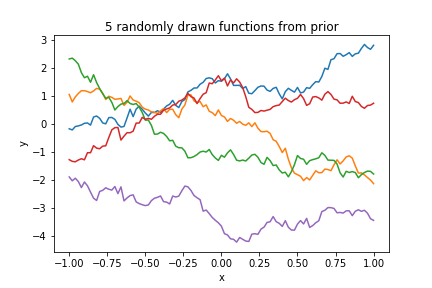
\includegraphics{../Figures/1.4.png}
		\caption{Results for 1.4; 5 randomly drawn functions drawn from the prior over the input space.}
		\label{fig:1.4}
	\end{figure}
	
    \begin{Verbatim}[commandchars=\\\{\}]
{\color{incolor}In [{\color{incolor}4}]:} \PY{c+c1}{\PYZsh{} q4}
        \PY{c+c1}{\PYZsh{} import multivariate normal object}
        \PY{k+kn}{from} \PY{n+nn}{scipy}\PY{n+nn}{.}\PY{n+nn}{stats} \PY{k}{import} \PY{n}{multivariate\PYZus{}normal} \PY{k}{as} \PY{n}{mv}
        \PY{c+c1}{\PYZsh{} define mu / sigma}
        \PY{n}{mu} \PY{o}{=} \PY{n}{zeros}\PY{p}{(}\PY{n+nb}{len}\PY{p}{(}\PY{n}{x}\PY{p}{)}\PY{p}{)}
        \PY{c+c1}{\PYZsh{} prior object}
        \PY{n}{prior} \PY{o}{=} \PY{n}{mv}\PY{p}{(}\PY{n}{mu}\PY{p}{,} \PY{n}{K}\PY{p}{)}
        \PY{c+c1}{\PYZsh{} sample from prior}
        \PY{n}{samples} \PY{o}{=} \PY{n}{prior}\PY{o}{.}\PY{n}{rvs}\PY{p}{(}\PY{l+m+mi}{5}\PY{p}{)}
        
\end{Verbatim}

    \begin{Verbatim}[commandchars=\\\{\}]
{\color{incolor}In [{\color{incolor}5}]:} \PY{c+c1}{\PYZsh{} show samples from the prior}
        \PY{n}{fig}\PY{p}{,} \PY{n}{ax} \PY{o}{=} \PY{n}{subplots}\PY{p}{(}\PY{l+m+mi}{1}\PY{p}{,} \PY{l+m+mi}{1}\PY{p}{)}
        \PY{k}{for} \PY{n}{i} \PY{o+ow}{in} \PY{n}{samples}\PY{p}{:}
            \PY{n}{ax}\PY{o}{.}\PY{n}{plot}\PY{p}{(}\PY{n}{x}\PY{p}{,} \PY{n}{i}\PY{p}{)}
        \PY{n}{savefig}\PY{p}{(}\PY{l+s+s1}{\PYZsq{}}\PY{l+s+s1}{../Figures/ex1q5}\PY{l+s+s1}{\PYZsq{}}\PY{p}{)}
        \PY{n}{ax}\PY{o}{.}\PY{n}{set\PYZus{}xlabel}\PY{p}{(}\PY{l+s+s1}{\PYZsq{}}\PY{l+s+s1}{x}\PY{l+s+s1}{\PYZsq{}}\PY{p}{)}
        \PY{n}{ax}\PY{o}{.}\PY{n}{set\PYZus{}ylabel}\PY{p}{(}\PY{l+s+s1}{\PYZsq{}}\PY{l+s+s1}{y}\PY{l+s+s1}{\PYZsq{}}\PY{p}{)}
        \PY{n}{ax}\PY{o}{.}\PY{n}{set\PYZus{}title}\PY{p}{(}\PY{l+s+s1}{\PYZsq{}}\PY{l+s+s1}{5 randomly drawn functions from prior}\PY{l+s+s1}{\PYZsq{}}\PY{p}{)}
        \PY{n}{savefig}\PY{p}{(}\PY{l+s+s1}{\PYZsq{}}\PY{l+s+s1}{../Figures/1.4.png}\PY{l+s+s1}{\PYZsq{}}\PY{p}{)}
\end{Verbatim}


	
    \subsection{5}\label{section}
	The code is self-explanatory; feed the kernel the training set with different theta values. The results are displayed in \ref{fig:1.5}.
	
    \begin{Verbatim}[commandchars=\\\{\}]
{\color{incolor}In [{\color{incolor}6}]:} \PY{c+c1}{\PYZsh{} q5}
        \PY{n}{thetas} \PY{o}{=} \PY{n}{np}\PY{o}{.}\PY{n}{array}\PY{p}{(}\PY{p}{[} \PY{p}{[} \PY{l+m+mi}{1}\PY{p}{,} \PY{l+m+mi}{4}\PY{p}{,} \PY{l+m+mi}{0}\PY{p}{,} \PY{l+m+mi}{0} \PY{p}{]}\PY{p}{,}\PYZbs{}
                           \PY{p}{[} \PY{l+m+mi}{9}\PY{p}{,} \PY{l+m+mi}{4}\PY{p}{,} \PY{l+m+mi}{0}\PY{p}{,} \PY{l+m+mi}{0} \PY{p}{]}\PY{p}{,}\PYZbs{}
                           \PY{p}{[} \PY{l+m+mi}{1}\PY{p}{,} \PY{l+m+mi}{64}\PY{p}{,} \PY{l+m+mi}{0}\PY{p}{,} \PY{l+m+mi}{0} \PY{p}{]}\PY{p}{,}
                         \PY{p}{[} \PY{l+m+mi}{1}\PY{p}{,} \PY{l+m+mf}{0.25}\PY{p}{,} \PY{l+m+mi}{0}\PY{p}{,} \PY{l+m+mi}{0} \PY{p}{]}\PY{p}{,}\PYZbs{}
                           \PY{p}{[} \PY{l+m+mi}{1}\PY{p}{,} \PY{l+m+mi}{4}\PY{p}{,} \PY{l+m+mi}{10}\PY{p}{,} \PY{l+m+mi}{0} \PY{p}{]}\PY{p}{,}\PYZbs{}
                           \PY{p}{[} \PY{l+m+mi}{1}\PY{p}{,} \PY{l+m+mi}{4}\PY{p}{,} \PY{l+m+mi}{0}\PY{p}{,} \PY{l+m+mi}{5} \PY{p}{]} \PY{p}{]}\PY{p}{)}
        
        \PY{c+c1}{\PYZsh{} we want at most 3 rows}
        \PY{n}{nRows} \PY{o}{=} \PY{l+m+mi}{3}
        \PY{c+c1}{\PYZsh{} get the the number of columns}
        \PY{n}{nCols} \PY{o}{=} \PY{n}{thetas}\PY{o}{.}\PY{n}{shape}\PY{p}{[} \PY{l+m+mi}{0} \PY{p}{]} \PY{o}{/}\PY{o}{/} \PY{n}{nRows}
        
        \PY{c+c1}{\PYZsh{} plot the prior for different theta}
        \PY{n}{fig}\PY{p}{,} \PY{n}{ax} \PY{o}{=} \PY{n}{subplots}\PY{p}{(}\PY{n}{nrows}\PY{o}{=}\PY{n}{nRows}\PY{p}{,} \PY{n}{ncols}\PY{o}{=}\PY{n}{nCols}\PY{p}{,} \PY{n}{sharex}\PY{o}{=}\PY{l+s+s1}{\PYZsq{}}\PY{l+s+s1}{all}\PY{l+s+s1}{\PYZsq{}}\PY{p}{)}
        \PY{k}{for} \PY{n}{idx}\PY{p}{,} \PY{n}{thetai} \PY{o+ow}{in} \PY{n+nb}{enumerate}\PY{p}{(}\PY{n}{thetas}\PY{p}{)}\PY{p}{:}
            \PY{c+c1}{\PYZsh{} compute the Gramm matrix}
            \PY{n}{K} \PY{o}{=} \PY{n}{kernel}\PY{p}{(}\PY{n}{x}\PY{p}{,} \PY{n}{x}\PY{p}{,} \PY{n}{thetai}\PY{p}{)}
            \PY{c+c1}{\PYZsh{} generate prior object}
            \PY{n}{prior} \PY{o}{=} \PY{n}{mv}\PY{p}{(}\PY{n}{mu}\PY{p}{,} \PY{n}{K}\PY{p}{,} \PY{n}{allow\PYZus{}singular}\PY{o}{=}\PY{l+m+mi}{1}\PY{p}{)}
            \PY{c+c1}{\PYZsh{} sample from the prior}
            \PY{n}{samples} \PY{o}{=} \PY{n}{prior}\PY{o}{.}\PY{n}{rvs}\PY{p}{(}\PY{l+m+mi}{5}\PY{p}{)}
            \PY{k}{for} \PY{n}{i} \PY{o+ow}{in} \PY{n}{samples}\PY{p}{:}
                \PY{n}{ax}\PY{o}{.}\PY{n}{flatten}\PY{p}{(}\PY{p}{)}\PY{p}{[} \PY{n}{idx} \PY{p}{]}\PY{o}{.}\PY{n}{plot}\PY{p}{(}\PY{n}{x}\PY{p}{,} \PY{n}{i}\PY{p}{)}
            \PY{n}{ax}\PY{o}{.}\PY{n}{flatten}\PY{p}{(}\PY{p}{)} \PY{p}{[} \PY{n}{idx} \PY{p}{]}\PY{o}{.}\PY{n}{set\PYZus{}title}\PY{p}{(}\PY{l+s+s1}{r\PYZsq{}}\PY{l+s+s1}{\PYZdl{}}\PY{l+s+s1}{\PYZbs{}}\PY{l+s+s1}{theta\PYZdl{} = }\PY{l+s+si}{\PYZob{}0\PYZcb{}}\PY{l+s+s1}{\PYZsq{}}\PY{o}{.}\PY{n}{format}\PY{p}{(}\PY{n}{thetai}\PY{p}{)}\PY{p}{)}
            \PY{n}{ax}\PY{o}{.}\PY{n}{flatten}\PY{p}{(}\PY{p}{)} \PY{p}{[} \PY{n}{idx} \PY{p}{]}\PY{o}{.}\PY{n}{set\PYZus{}xlabel}\PY{p}{(}\PY{l+s+s1}{\PYZsq{}}\PY{l+s+s1}{x}\PY{l+s+s1}{\PYZsq{}}\PY{p}{)}
            \PY{n}{ax}\PY{o}{.}\PY{n}{flatten}\PY{p}{(}\PY{p}{)} \PY{p}{[} \PY{n}{idx} \PY{p}{]}\PY{o}{.}\PY{n}{set\PYZus{}ylabel}\PY{p}{(}\PY{l+s+s1}{\PYZsq{}}\PY{l+s+s1}{y}\PY{l+s+s1}{\PYZsq{}}\PY{p}{)}
        \PY{n}{fig}\PY{o}{.}\PY{n}{suptitle}\PY{p}{(}\PY{l+s+s1}{r\PYZsq{}}\PY{l+s+s1}{Samples from prior with different \PYZdl{}}\PY{l+s+s1}{\PYZbs{}}\PY{l+s+s1}{theta\PYZdl{} }\PY{l+s+s1}{\PYZsq{}}\PY{p}{)}
        \PY{n}{fig}\PY{o}{.}\PY{n}{tight\PYZus{}layout}\PY{p}{(}\PY{p}{)}
        \PY{n}{fig}\PY{o}{.}\PY{n}{subplots\PYZus{}adjust}\PY{p}{(}\PY{n}{top}\PY{o}{=}\PY{l+m+mf}{0.85}\PY{p}{)}
        \PY{n}{savefig}\PY{p}{(}\PY{l+s+s1}{\PYZsq{}}\PY{l+s+s1}{../Figures/1.5.png}\PY{l+s+s1}{\PYZsq{}}\PY{p}{)}
\end{Verbatim}

	\begin{figure}[H]
	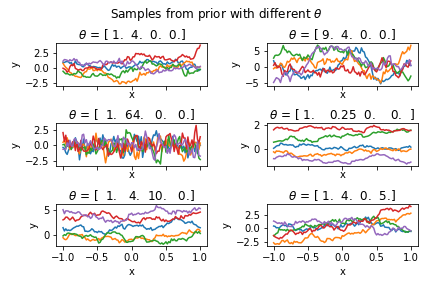
\includegraphics{../Figures/1.5.png}
	\caption{Results for 1.5. Samples drawn from the prior for different values of theta. An explanation for the different settings of $\theta$ is given in \ref{bonus-explanation}.}
	\end{figure}

    \subsubsection{Bonus explanation}\label{bonus-explanation} 

From the left column top two plots, and middle right we see that
\(\theta[1]\) regulates the amount of `jitter' in the random process.
From (3) we see that \(\theta[1]\) weighs the euclidean distance between
\(x, x'\). Comparing the top row plots, we see that the non-linearity of
the random process is controlled by increasing \(\theta[0]\), i.e.
(global) curvature of the lines. In other words, the gaussian part of the kernel favors clustered points, i.e. if the euclidean distance between them is small, it will tend to pull the process towards these points; creating these jitters we see here.  The off-set of the random process is
controlled by \(\theta[2]\) (trivially) this can be seen in comparing
the bottom and top plot in the left column. Finally, \(\theta[3]\)
controls the amount of linearity of change in the random process. This
can be seen in bottom right plot, compared to the top row of plots. So
in all we can summarize it as:

\begin{enumerate}
  \item - Given the kernel function in (3):
  \begin{itemize}
  \item  $\theta[0]$ controls the non-linear component of the random process

  \item  $\theta[1]$ controls the 'jitterness' of the random process, i.e. weigh the euclidean distance in the random process

  \item $\theta[2]$ controls the mean off set in the random process

  \item $\theta[3]$ controls the linear component of change of the random process
  \end{itemize}
\end{enumerate}

    \subsection{6}\label{section}

    In computing C we will use equation 6.62 from Bisschop.

    \begin{Verbatim}[commandchars=\\\{\}]
{\color{incolor}In [{\color{incolor}7}]:} \PY{c+c1}{\PYZsh{} q6}
        \PY{c+c1}{\PYZsh{} define training set; inputs, targets}
        \PY{n}{xTrain} \PY{o}{=} \PY{n}{array}\PY{p}{(}\PY{p}{[}\PY{p}{[}\PY{o}{\PYZhy{}}\PY{o}{.}\PY{l+m+mi}{5}\PY{p}{,} \PY{o}{.}\PY{l+m+mi}{2}\PY{p}{,} \PY{o}{.}\PY{l+m+mi}{3} \PY{p}{,} \PY{o}{\PYZhy{}}\PY{o}{.}\PY{l+m+mi}{1}\PY{p}{]}\PY{p}{]}\PY{p}{)}\PY{o}{.}\PY{n}{T}
        \PY{n}{tTrain} \PY{o}{=} \PY{n}{array}\PY{p}{(}\PY{p}{[}\PY{p}{[}\PY{o}{.}\PY{l+m+mi}{5}\PY{p}{,} \PY{o}{\PYZhy{}}\PY{l+m+mi}{1}\PY{p}{,} \PY{l+m+mi}{3}\PY{p}{,} \PY{o}{\PYZhy{}}\PY{l+m+mf}{2.5}\PY{p}{]}\PY{p}{]}\PY{p}{)}\PY{o}{.}\PY{n}{T}
        \PY{n}{KTrain} \PY{o}{=} \PY{n}{kernel}\PY{p}{(}\PY{n}{xTrain}\PY{p}{,} \PY{n}{xTrain}\PY{p}{,} \PY{n}{theta}\PY{p}{)}
        \PY{n}{beta}   \PY{o}{=} \PY{l+m+mi}{1}
        \PY{n}{C}      \PY{o}{=} \PY{n}{KTrain} \PY{o}{+} \PY{l+m+mi}{1}\PY{o}{/}\PY{n}{beta} \PY{o}{*} \PY{n}{eye}\PY{p}{(}\PY{n+nb}{len}\PY{p}{(}\PY{n}{xTrain}\PY{p}{)}\PY{p}{)}
        \PY{n+nb}{print}\PY{p}{(}\PY{l+s+s1}{\PYZsq{}}\PY{l+s+s1}{C:}\PY{l+s+se}{\PYZbs{}n}\PY{l+s+s1}{ }\PY{l+s+s1}{\PYZsq{}}\PY{p}{,}\PY{n}{C}\PY{p}{)}
        
        \PY{c+c1}{\PYZsh{} show the training points}
        \PY{n}{fig}\PY{p}{,} \PY{n}{ax} \PY{o}{=} \PY{n}{subplots}\PY{p}{(}\PY{p}{)}
        \PY{n}{ax}\PY{o}{.}\PY{n}{scatter}\PY{p}{(}\PY{n}{xTrain}\PY{p}{,} \PY{n}{tTrain}\PY{p}{)}
        \PY{n}{ax}\PY{o}{.}\PY{n}{set\PYZus{}title}\PY{p}{(}\PY{l+s+s1}{\PYZsq{}}\PY{l+s+s1}{Scatter plot of training points}\PY{l+s+s1}{\PYZsq{}}\PY{p}{)}
        \PY{n}{ax}\PY{o}{.}\PY{n}{set\PYZus{}ylabel}\PY{p}{(}\PY{l+s+s1}{\PYZsq{}}\PY{l+s+s1}{Targets}\PY{l+s+s1}{\PYZsq{}}\PY{p}{)}
        \PY{n}{ax}\PY{o}{.}\PY{n}{set\PYZus{}xlabel}\PY{p}{(}\PY{l+s+s1}{\PYZsq{}}\PY{l+s+s1}{Input}\PY{l+s+s1}{\PYZsq{}}\PY{p}{)}
        \PY{n}{savefig}\PY{p}{(}\PY{l+s+s1}{\PYZsq{}}\PY{l+s+s1}{../Figures/1.6.png}\PY{l+s+s1}{\PYZsq{}}\PY{p}{)}
\end{Verbatim}

    \begin{Verbatim}[commandchars=\\\{\}]
C:
  [[ 3.25        1.60468809  1.52032005  1.86873075]
 [ 1.60468809  3.04        2.01122942  1.84070798]
 [ 1.52032005  2.01122942  3.09        1.78873075]
 [ 1.86873075  1.84070798  1.78873075  3.01      ]]

    \end{Verbatim}

    \section{7}\label{section}

    In order to compute the \(\mu\) at x = 0, we will to compute the Gramm
matrix using the training points and the new point (see Bisschop p.307);
i.e.~we compute \emph{K} =
K(\(\boldsymbol{X_n}, \boldsymbol{X_{N+1}}\)), where
\(\boldsymbol{X_n}\) is the set \(i = 1,...,N\) and \(X_{N+1} = 0\).

    \begin{Verbatim}[commandchars=\\\{\}]
{\color{incolor}In [{\color{incolor}8}]:} \PY{n}{xNew}       \PY{o}{=} \PY{n}{array}\PY{p}{(}\PY{p}{[}\PY{p}{[}\PY{l+m+mi}{0}\PY{p}{]}\PY{p}{]}\PY{p}{)}
        \PY{n}{xTrainNew}  \PY{o}{=} \PY{n}{vstack}\PY{p}{(}\PY{p}{(}\PY{n}{xTrain}\PY{p}{,} \PY{n}{xNew}\PY{p}{)}\PY{p}{)}
        \PY{n}{c}          \PY{o}{=} \PY{n}{kernel}\PY{p}{(}\PY{n}{xNew}\PY{p}{,} \PY{n}{xNew}\PY{p}{,} \PY{n}{theta}\PY{p}{)} \PY{o}{+} \PY{l+m+mi}{1}\PY{o}{/}\PY{n}{beta}
        \PY{n}{k}          \PY{o}{=} \PY{n}{kernel}\PY{p}{(}\PY{n}{xTrain}\PY{p}{,} \PY{n}{xNew}\PY{p}{,} \PY{n}{theta}\PY{p}{)}
        \PY{n}{invC}       \PY{o}{=} \PY{n}{linalg}\PY{o}{.}\PY{n}{inv}\PY{p}{(}\PY{n}{C}\PY{p}{)}
        \PY{c+c1}{\PYZsh{} Bisschop 6.66}
        \PY{n}{mu\PYZus{}new}     \PY{o}{=} \PY{n}{k}\PY{o}{.}\PY{n}{T}\PY{o}{.}\PY{n}{dot}\PY{p}{(}\PY{n}{invC}\PY{p}{)}\PY{o}{.}\PY{n}{dot}\PY{p}{(}\PY{n}{tTrain}\PY{p}{)}
        \PY{c+c1}{\PYZsh{} Bisschop 6.67}
        \PY{n}{sigma\PYZus{}new}  \PY{o}{=} \PY{n}{c} \PY{o}{\PYZhy{}} \PY{n}{k}\PY{o}{.}\PY{n}{T}\PY{o}{.}\PY{n}{dot}\PY{p}{(}\PY{n}{invC}\PY{p}{)}\PY{o}{.}\PY{n}{dot}\PY{p}{(}\PY{n}{k}\PY{p}{)}
        \PY{n+nb}{print}\PY{p}{(}\PY{l+s+s1}{\PYZsq{}}\PY{l+s+s1}{mu at x = }\PY{l+s+si}{\PYZob{}0\PYZcb{}}\PY{l+s+s1}{:}\PY{l+s+se}{\PYZbs{}n}\PY{l+s+si}{\PYZob{}1\PYZcb{}}\PY{l+s+s1}{\PYZsq{}}\PY{o}{.}\PY{n}{format}\PY{p}{(}\PY{n}{xNew}\PY{p}{[}\PY{l+m+mi}{0}\PY{p}{]}\PY{p}{,} \PY{n}{mu\PYZus{}new}\PY{p}{)} \PY{p}{)}
        \PY{n+nb}{print}\PY{p}{(}\PY{l+s+s1}{\PYZsq{}}\PY{l+s+s1}{sigma\PYZca{}2 at x = }\PY{l+s+si}{\PYZob{}0\PYZcb{}}\PY{l+s+s1}{:}\PY{l+s+se}{\PYZbs{}n}\PY{l+s+si}{\PYZob{}1\PYZcb{}}\PY{l+s+s1}{\PYZsq{}}\PY{o}{.}\PY{n}{format}\PY{p}{(}\PY{n}{xNew}\PY{p}{[}\PY{l+m+mi}{0}\PY{p}{]}\PY{p}{,} \PY{n}{sigma\PYZus{}new}\PY{p}{)} \PY{p}{)}
\end{Verbatim}

    \begin{Verbatim}[commandchars=\\\{\}]
mu at x = [0]:
[[-0.20721389]]
sigma\^{}2 at x = [0]:
[[ 1.32520089]]

    \end{Verbatim}

    \section{8}\label{section}

    The mean of \(p(t \mid \boldsymbol(t)))\) will not go to zero as
\(x \rightarrow \pm \infty\). If \(x\) approaches \(\pm \infty\) the
gaussian part of (3) will go to zero but the linear part (\(x^T x'\))
will blow up to \(\pm \infty\) (depending on the sign of \(x, x'\) ( for more in depth explanation please see the bonus question above). Thus to
make the kernel function to go to zero we would need to suppress
\(x^T x'\) by setting \(\theta[3] = \theta[2] = 0\) (the bias,
\(\theta[2]\) will trivially cause non-zero if set to anything else than
zero).

As an example, we take a large value for x and print the mean by setting
\(\theta[2] = \theta[3] = 0\).

    \begin{Verbatim}[commandchars=\\\{\}]
{\color{incolor}In [{\color{incolor}9}]:} \PY{c+c1}{\PYZsh{} take a very large number}
        \PY{n}{xNew}       \PY{o}{=} \PY{n}{array}\PY{p}{(}\PY{p}{[}\PY{p}{[}\PY{l+m+mi}{1}\PY{n}{e30}\PY{p}{]}\PY{p}{]}\PY{p}{)}
        \PY{n}{xTrainNew}  \PY{o}{=} \PY{n}{vstack}\PY{p}{(}\PY{p}{(}\PY{n}{xTrain}\PY{p}{,} \PY{n}{xNew}\PY{p}{)}\PY{p}{)}
        \PY{n}{c}          \PY{o}{=} \PY{n}{kernel}\PY{p}{(}\PY{n}{xNew}\PY{p}{,} \PY{n}{xNew}\PY{p}{,} \PY{n}{theta}\PY{p}{)} \PY{o}{+} \PY{l+m+mi}{1}\PY{o}{/}\PY{n}{beta}
        \PY{n}{thetaEdit}  \PY{o}{=} \PY{n}{theta}\PY{o}{.}\PY{n}{copy}\PY{p}{(}\PY{p}{)}
        \PY{n}{thetaEdit}\PY{p}{[}\PY{o}{\PYZhy{}}\PY{l+m+mi}{2}\PY{p}{:}\PY{p}{]} \PY{o}{=} \PY{l+m+mi}{0}
        \PY{n}{k}          \PY{o}{=} \PY{n}{kernel}\PY{p}{(}\PY{n}{xTrain}\PY{p}{,} \PY{n}{xNew}\PY{p}{,} \PY{n}{thetaEdit}\PY{p}{)}
        \PY{n}{invC}       \PY{o}{=} \PY{n}{linalg}\PY{o}{.}\PY{n}{inv}\PY{p}{(}\PY{n}{C}\PY{p}{)}
        \PY{c+c1}{\PYZsh{} Bisschop 6.66}
        \PY{n}{mu\PYZus{}new}     \PY{o}{=} \PY{n}{k}\PY{o}{.}\PY{n}{T}\PY{o}{.}\PY{n}{dot}\PY{p}{(}\PY{n}{invC}\PY{p}{)}\PY{o}{.}\PY{n}{dot}\PY{p}{(}\PY{n}{tTrain}\PY{p}{)}
        \PY{c+c1}{\PYZsh{} Bisschop 6.67}
        \PY{n}{sigma\PYZus{}new}  \PY{o}{=} \PY{n}{c} \PY{o}{\PYZhy{}} \PY{n}{k}\PY{o}{.}\PY{n}{T}\PY{o}{.}\PY{n}{dot}\PY{p}{(}\PY{n}{invC}\PY{p}{)}\PY{o}{.}\PY{n}{dot}\PY{p}{(}\PY{n}{k}\PY{p}{)}
        \PY{n+nb}{print}\PY{p}{(}\PY{l+s+s1}{\PYZsq{}}\PY{l+s+s1}{mu at x  = }\PY{l+s+si}{\PYZob{}0\PYZcb{}}\PY{l+s+s1}{:}\PY{l+s+se}{\PYZbs{}n}\PY{l+s+si}{\PYZob{}1\PYZcb{}}\PY{l+s+se}{\PYZbs{}n}\PY{l+s+s1}{and theta:}\PY{l+s+se}{\PYZbs{}n}\PY{l+s+s1}{ }\PY{l+s+si}{\PYZob{}2\PYZcb{}}\PY{l+s+s1}{\PYZsq{}}\PYZbs{}
              \PY{o}{.}\PY{n}{format}\PY{p}{(}\PY{n}{xNew}\PY{p}{[}\PY{l+m+mi}{0}\PY{p}{]}\PY{p}{,} \PY{n}{mu\PYZus{}new}\PY{p}{,} \PY{n}{thetaEdit}\PY{p}{)} \PY{p}{)}
\end{Verbatim}

    \begin{Verbatim}[commandchars=\\\{\}]
mu at x  = [  1.00000000e+30]:
[[ 0.]]
and theta:
 [ 1.  1.  0.  0.]

    \end{Verbatim}


    % Add a bibliography block to the postdoc
    
    
    
    \end{document}
